\newcommand{\institut}{}
\newcommand{\fachgebiet}{Regelungstechnik}
\newcommand{\veranstaltung}{Praktikum Grundlagen der Regelungstechnik}
\newcommand{\pdfautor}{Dirk Barbendererde (321 836), Boris Henckell (325 779)}
\newcommand{\autor}{Dirk Barbendererde (321 836)\\ Boris Henckell (325 779)}
\newcommand{\pdftitle}{Praktikum\ Regelungstechnik\ Versuch\ 3}
\newcommand{\prototitle}{Praktikum Regelungstechnik \\ Versuch 3}
\newcommand{\aufgabe}{}

\newcommand{\gruppe}{Gruppe: G1 Di 12-14}
\newcommand{\betreuer}{Betreuer: Markus Valtin}



\input{../../packages/tu_header_9}
\begin{document}


%     \lstinputlisting{./praktikum6.sce}



%---------------------------------------------------------------------
%---------------------------------------------------------------------
%---------------------------------------------------------------------

\section{Reglerentwurf}
\begin{quote}
	\hspace{-2em}
	\subsection{PID-Regler}
	\label{aufg:3.1}
	
	Aufgabe:\\
	Entwerfen Sie für das totzeitfreie System
	
	\begin{equation*}
    	\begin{split}
    		\tilde{G}(s) = \frac{V_0}{(s-s_{\infty 1})(s-s_{\infty 2})}
    	\end{split}
    \end{equation*}
	
	einen (realen) PID-Regler $K_{PID}$, indem sie beide Polstellen der Strecke kürzen. Die übrigen Parameter sollen so
	bestimmt werden, dass die Dynamik des Führungsverhaltens des resultierenden Regelkreises mit dem des folgenden Polpaares übereinstimmt:
	
	\begin{equation*}
    	\begin{split}
    		P(s) = \frac{1}{s^2 \omega^2 + s \frac{2 d}{\omega} + 1}
    	\end{split}
    \end{equation*}
	
	Der Regelkreis soll also relativ schnell sein, jedoch ohne dass dabei Überschwingen auftritt.\vspace{1em}
	
    \begin{quote}
        
        Zu Beginn des Reglerentwurfs definieren wir die uns vorgegebene linearisierte Stecke $\tilde{G}$.\\
        Anschließend erstellen wir folgendermaßen unseren PID-Regler:
        \begin{equation*}
        	\begin{split}
        		\tilde{K} &= K_{PID} \  \frac{1}{1 + T s} \ \frac{1}{s} (s^2  T_d T_i + T_i s + 1)\\
        	\end{split}
        \end{equation*}
        
        mit 
        
        \begin{equation*}
        	\begin{split}
        		T_i &= \frac{-(s_1 + s_2)}{s_1 s_2}\\
        		T_d &= \frac{1}{-(s_1 + s_2)}\\
        	\end{split}
        \end{equation*}
        
        In diesem Fall stellen die beiden Variablen $s_1$ und $s_2$ die Polstellen der Strecke $\tilde{G}$ dar. Auf
        diese Weise kürzen wir diese schon mal durch den Regeler. Verbleiben noch die Position des Realisierbarkeitspols
        sowie die Verstärkung des Reglers als Parameter um die Dynamik des Führungsverhaltens des Reglers zu
        beeinflussen.\\
        
        Als Vergleich erstellen wir die Führungssprungantwort des gegebenen Polpaars.\\
        
        Mit einer Versärkung von $K_{PID} = 1.6$ und einem Realisierbarkeitspol bei $-20$ erhalten wir folgende
        Führungssprünge:
        
        \begin{figure}[H]
        \centering
            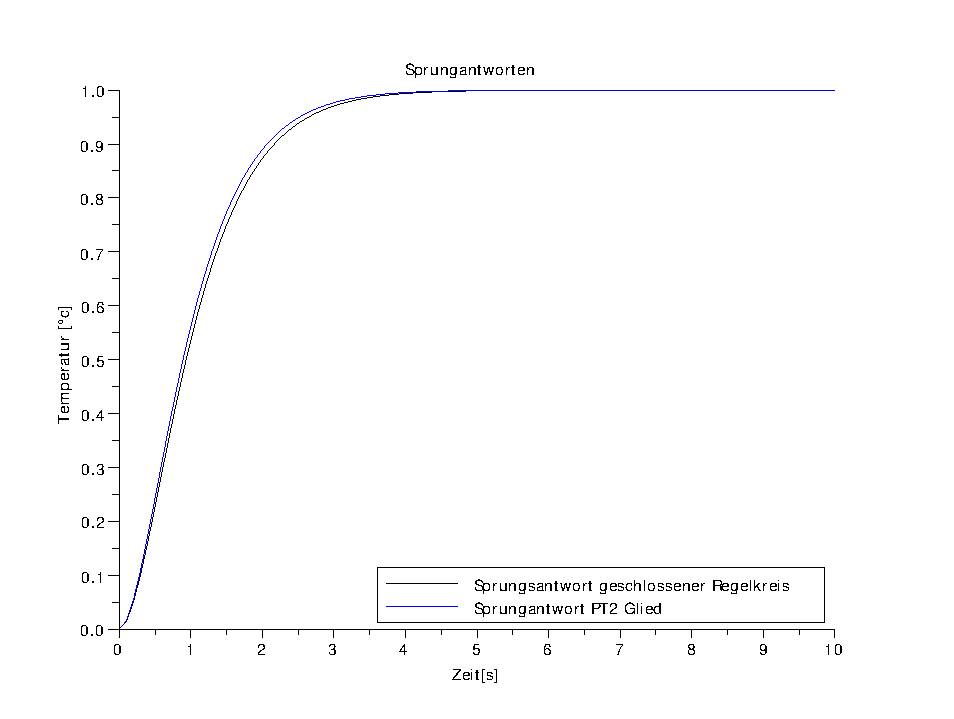
\includegraphics[scale=0.7, trim = 0cm 0cm 0cm 0cm, clip]{./Bilder/Sprungantwort}
                \caption{Führungssprungantwort}
        \end{figure}
    
    \end{quote}
    
    
    \subsection{Pad\'e-Approximation}
    
    Aufgabe:\\
    Approximieren Sie den Term $e^{-sT_d}$, welcher für die Totzeit verantwortlich ist, mithilfe einer
    Pad\'e-Approximation erster Ordnung durch eine gebrochen-rationale Funktion und stellen Sie das approximierte
    Streckenmodell $\tilde{G}$ auf, indem Sie die Totzeit in $G$ durch ihre Approximation ersetzen. \vspace{1em}
    
    \begin{quote}
        
        Als nächstes haben wir die Totzeit mit einer Pad\'e-Approximation erster Ordnung durch eine gebrochen-rationale
        Funktion ersetzt und multiplizieren sie an unsere Strecke. Für diese Näherung des Systems ($\hat{G}$) entwerfen
        wir nun einen Regler.\vspace{1em}
        
        Die Approximation lautet:
        \begin{equation*}
        	\begin{split}
        		p_1(s) = \frac{1-\frac{\tau}{2}s}{1+\frac{\tau}{2}s}
        	\end{split}
        \end{equation*}
        
    \end{quote}
    
    \subsection{Reglerentwurf für die Strecke $\hat{G}$}
    Aufgabe:\\
    Es soll ein Regler für das approximierte Streckenmodell $\hat{G}$ mittels Polvorgabe entworfen werden, der
    folgende Eigenschaften des geschlossenen Kreises ermöglicht:
        
        \begin{itemize}
            
            \item kein Überschwingen der Regelgröße bei sprungförmigen Führungs- oder Störsignalen
            
            \item ungefähr gleiche Anstiegszeit der Regelgröße wie bei der Verwendung des PID-Regler aus \ref{aufg:3.1}
            
            \item Regelfehler $\to$ 0 für t $\to$ $\infty$ unter sprungförmigen Referenzen
        
        \end{itemize}
        \vspace{1em}
        
        \begin{enumerate}
            
            \item Stellen Sie den Regleransatz mit kleinstmöglicher Nennerordnung und Integratoranteil auf. Wie viele Pole
            müssen Sie vorgeben?
            
            \item Stellen Sie das Sollpolpolynom auf; verwenden sie hierzu die Pole des Polpaares aus Aufgabe \ref{aufg:3.1}
            und die Pole der Strecke $G$, wählen sie einen weiteren Pol bei ($s_\infty = -2$).
            
            \item Stellen Sie die Sylvester Matrix durch Koeffizientenvergleich des Polpolynoms des geschlossenen Kreises
            mit Ihrem Sollpolpolynom auf und berechnen sie die Reglerparameter mithilfe von Scilab.
        
        \end{enumerate}\vspace{1em}
       
        Mit dem Regleransatz\\
        
        \begin{equation*}
            \begin{split}
                K(s) = \frac{\beta_0 + \beta_1 s + \beta_2 s^2 + \beta_3 s^3}{s(\alpha_0 + \alpha_1 s + s^2)}
            \end{split}
        \end{equation*}\vspace{1em}
        
    \begin{quote}
      
        Das approximierte Streckenmodell $\hat{G}$ allein hat die Ordnung $n = 3$. Da der Regler einen
        Integratoranteil besitzen soll und wir den Reglerentwurf wählen bei dem dieser Integrator im nachhinein
        an einen Regler multipliziert wird, müssen wir die Strecke anpassen und erhalten eine neue Streckenordnung von
        $n = 4$. Daraus folgt, dass die zu berechnende Sylvestermatrix $8\cdot 8$ Einträge und das Sollpolynom 8
        Einträge besitzen muss. Um das zu realisieren müssen wir insgesamt 7 Pole vorgeben, da der letzte Eintrag des
        Sollpolynoms der Koeffizent vor dem $s^0$ ist.\\
        
        Neben dem Pol bei $s_\infty = -2$ und den zwei Polen des Polpaares benötigen wir noch genau 4 Pole aus der
        veränderten Strecke. Unsere Strecke ergibt sich aus:
        
        \begin{equation*}
        	\begin{split}
        		\hat{G_I} = \hat{G} \frac{1}{s}
        	\end{split}
        \end{equation*}
        
        und hat genau 4 Pole.\\
        
        Insgesamt ergibt sich daraus das folgende Sollpolpolynom:
        
        \begin{equation*}
        	\begin{split}
        		q_{soll} = 32.148065s + 177.77307s^2 + 285.03595s^3 + 208.51884s^4 + 77.572633s^5 + 14.179911s^6 + s^7  
        	\end{split}
        \end{equation*}
        \vspace{1em}
        
        Anschließend haben wir die Sylvestermatrix aufgestellt und mithilfe des Sollpolpolynoms die Koeffizenten des
        Reglers errechnet.\\
        Unser Regler sieht folgendermaßen aus:
        
        \begin{equation*}
        	\begin{split}
        		KposI = \frac{14.231104 +  56.480246s +  26.455258s^2 +  3.1456906s^3}{62.570515s +  28.849556s^2 +  5s^3}
        	\end{split}
        \end{equation*}
        
        Damit entspricht er dem geforderten Regleransatz.\\
        Die Kontrolle der Polstellen des resultierenden geschlossenen Regelkreises ergibt, dass sie mit denen des
        Sollpolpolynoms übereinstimmen.
    \end{quote}
    
    
    
    \subsection{Smith-Prädiktor}
    Aufgabe:\\
    Entwerfen Sie für die totzeitbehaftete Strecke einen Smith-Prädiktor unter Verwendung des Reglers aus
    \ref{aufg:3.1}\vspace{1em}
    
    
    \begin{quote}
        
        Der Smith-Prädiktor für die totzeitbehaftete Strecke einen unter Verwendung des Reglers aus \ref{aufg:3.1} ergab sich wie folgt:
        
       \begin{figure}[H]
        \centering
            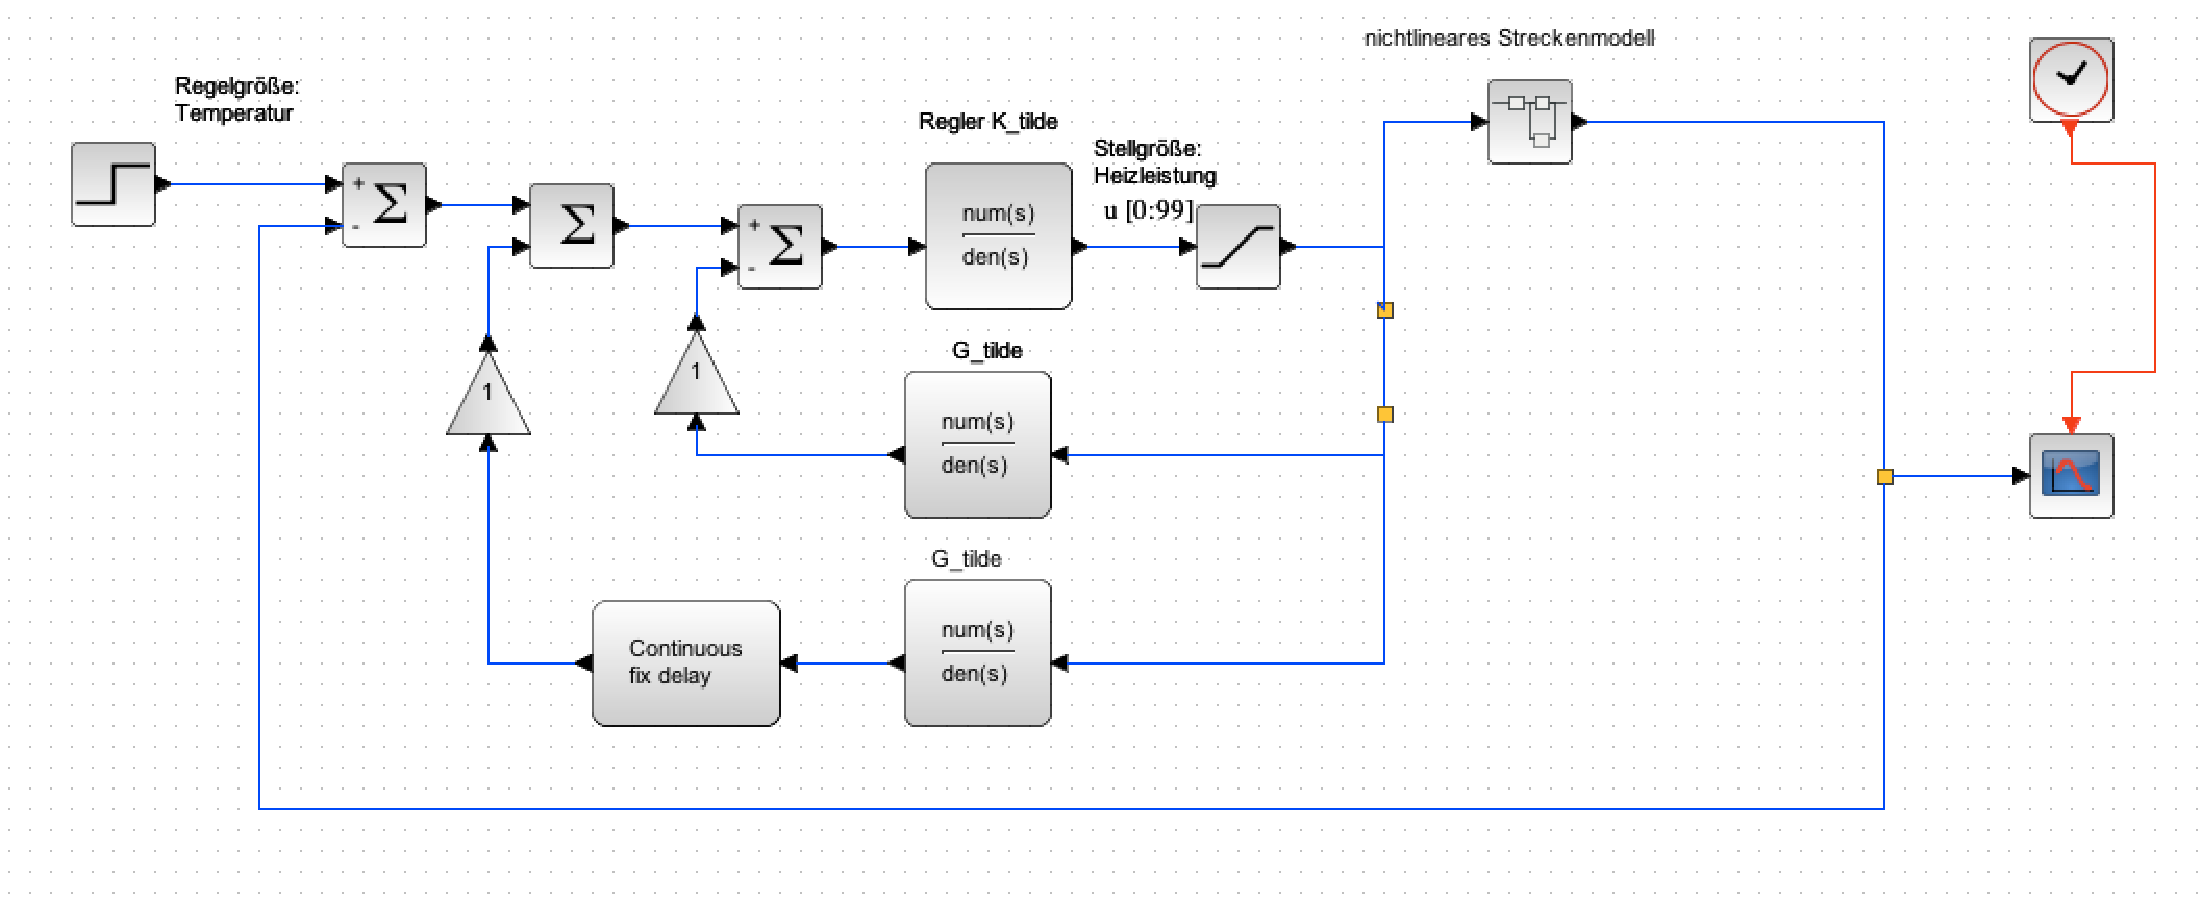
\includegraphics[scale=0.4, trim = 0cm 0cm 0cm 0cm, clip]{./Bilder/Smith-Praediktor}
                \caption{Smith-Prädiktor}
        \end{figure}
    
        
    \end{quote}
    
\end{quote} %Ende Section Reglerentwurf 

%--------------------------------------------------------------------
%--------------------------------------------------------------------


\section{Simulation}
\begin{quote}
    
    
    
    \subsection{Stabilität mit steigender Totzeit}
    \begin{quote}
        
    \end{quote}
    Aufgabe:%\\
    Simulieren Sie den PID Regler zunächst ohne Totzeit mit einem Führungssprung der Amplitude $+30^{\circ}C$ mit dem
    idealen $PT2$-Modell! Fügen Sie dem Modell solange größer werdende Totzeiten ($T_d = 0.4, 0.8, . . .$) hinzu, bis
    der Regelkreis instabil wird! Beschreiben Sie kurz, welchen Einfluss die Totzeit auf das Regelkreisverhalten
    hat!%\vspace{1em}
    
    \begin{quote}
            \begin{center}
                \begin{tabular}{ll}
                
                \hspace{-1cm}
                    \begin{minipage}{0.6\textwidth}
                        \begin{figure}[H]
                            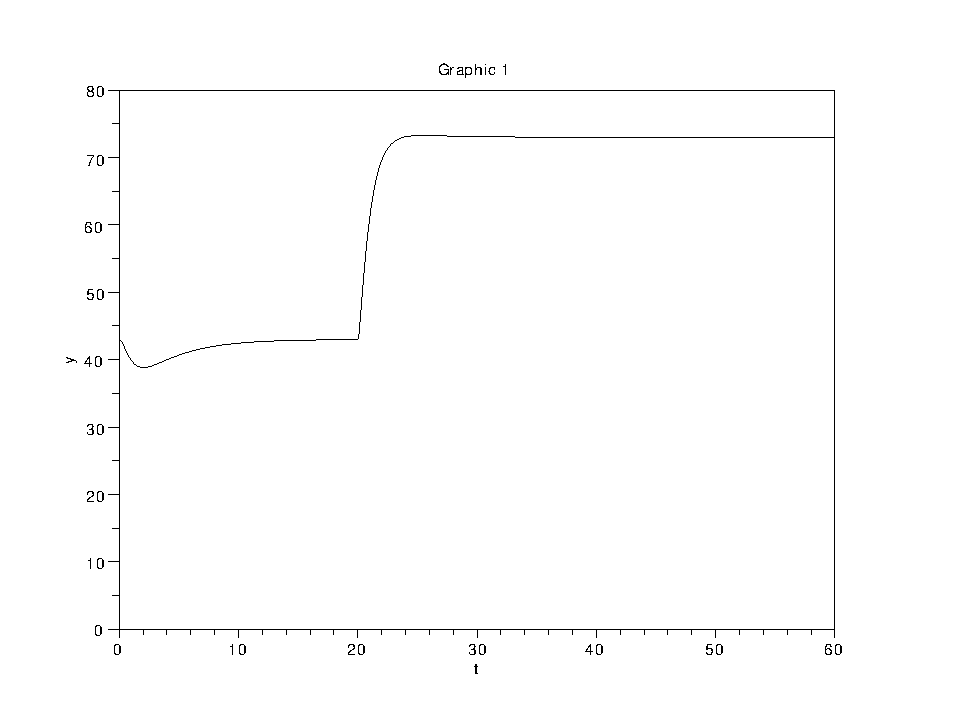
\includegraphics[scale=0.4, trim = 0cm 0cm 0cm
                            0cm, clip]
                            {./Bilder/4_1_Td_0}
                              \caption{Sprungantwort PID Regler lin. Modell Totzeit $T_d$ = 0}
                        \end{figure}
                    \end{minipage}
                    
                    \begin{minipage}{0.6\textwidth}
                        \begin{figure}[H]
                            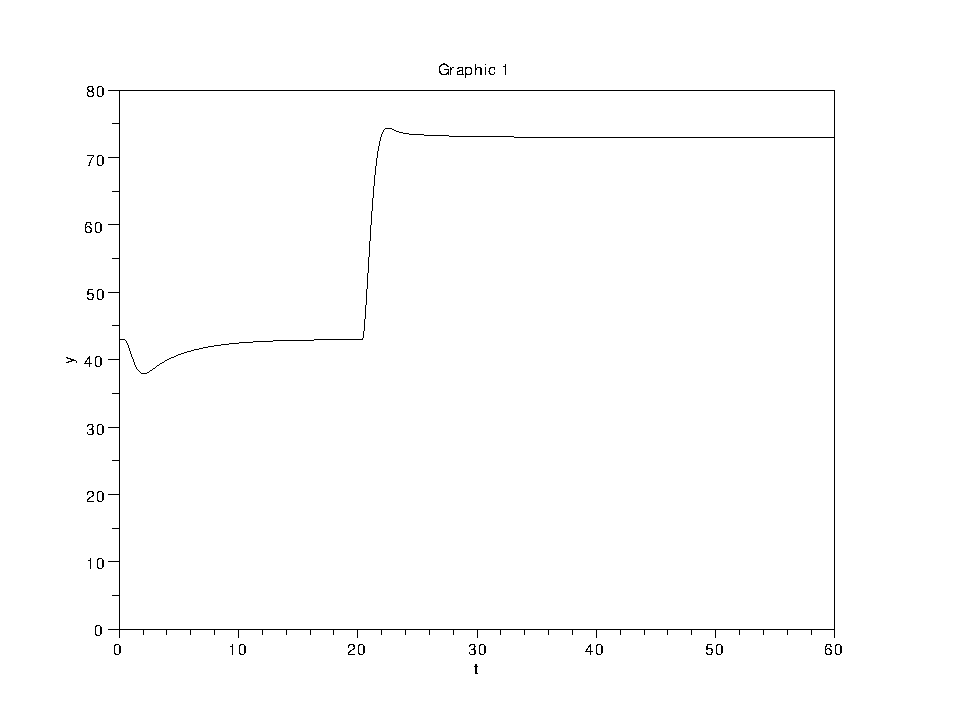
\includegraphics[scale=0.4,trim = 0cm 0cm 0cm
                            0cm, clip]
                            {./Bilder/4_1_Td_04}
                              \caption{Sprungantwort PID Regler lin. Modell Totzeit $T_d$ = 0.4}
                        \end{figure}
                    \end{minipage}
                
                \end{tabular}
            \end{center}

            \begin{center}
                \begin{tabular}{ll}
                
                \hspace{-1cm}
                    \begin{minipage}{0.6\textwidth}
                        \begin{figure}[H]
                            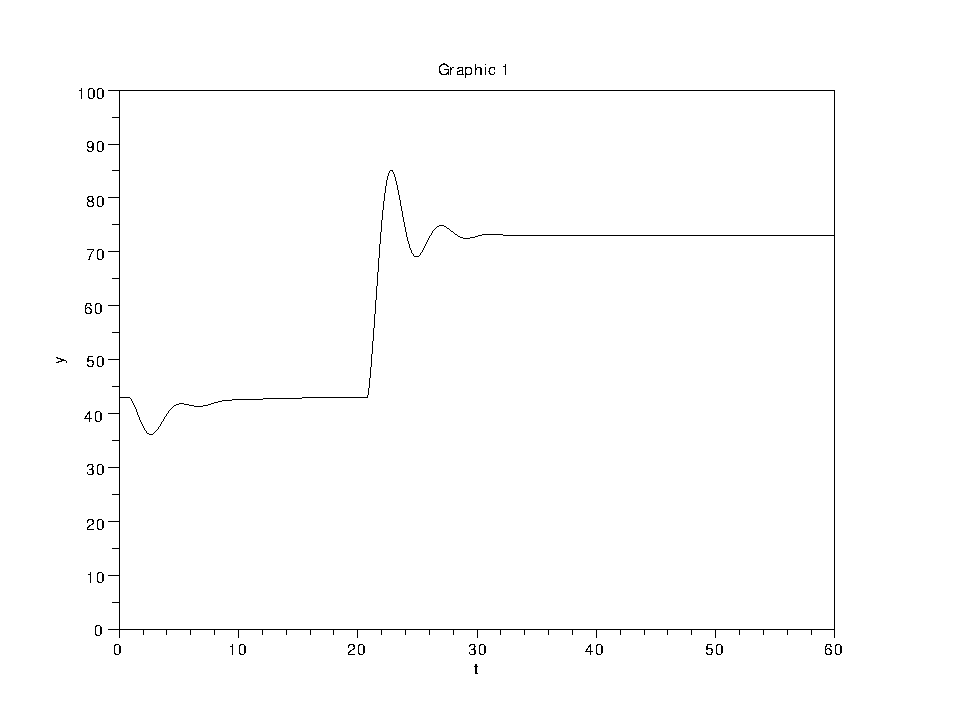
\includegraphics[scale=0.4, trim = 0cm 0cm 0cm
                            0cm, clip]
                            {./Bilder/4_1_Td_08}
                              \caption{Sprungantwort PID Regler lin. Modell Totzeit $T_d = 0.8$}
                        \end{figure}
                    \end{minipage}
                    
                    \begin{minipage}{0.6\textwidth}
                        \begin{figure}[H]
                            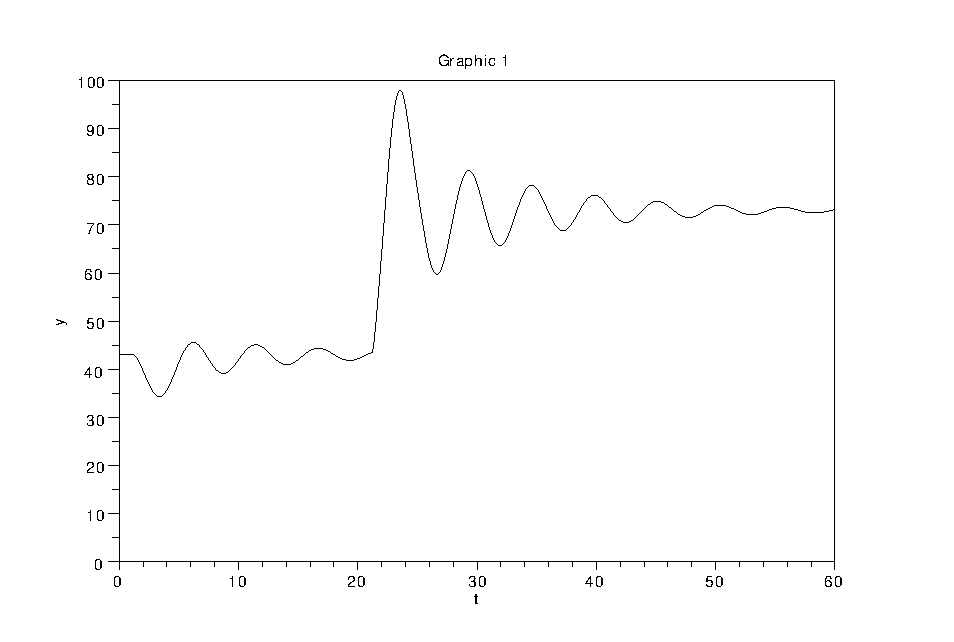
\includegraphics[scale=0.4,trim = 0cm 0cm 0cm
                            0cm, clip]
                            {./Bilder/4_1_Td_12}
                              \caption{Sprungantwort PID Regler lin. Modell Totzeit $T_d = 1.2$}
                        \end{figure}
                    \end{minipage}
                
                \end{tabular}
            \end{center}

            \begin{center}
                \begin{tabular}{ll}
                
                \hspace{-1cm}
                    \begin{minipage}{0.6\textwidth}
                        \begin{figure}[H]
                            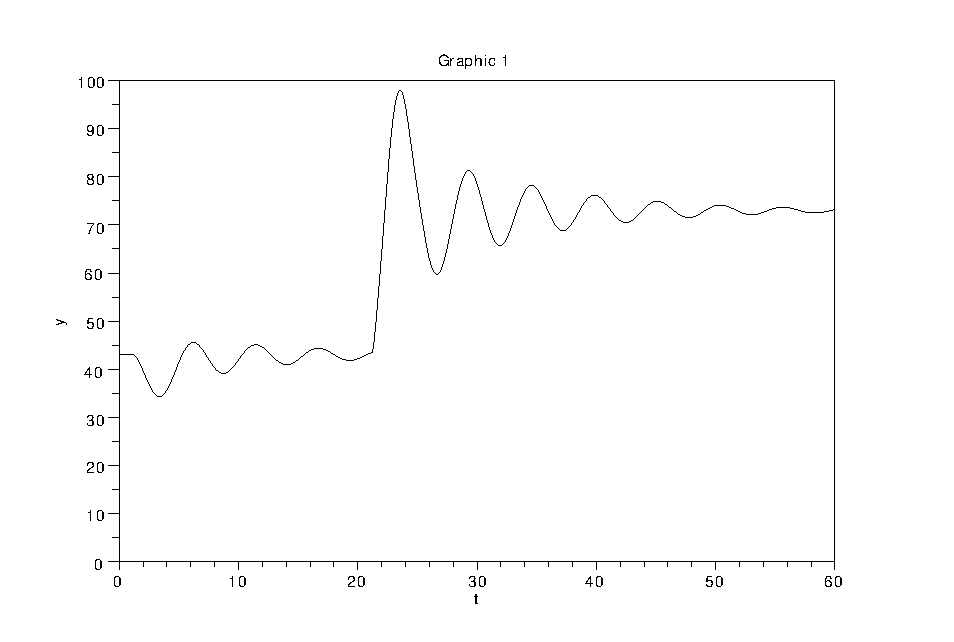
\includegraphics[scale=0.4, trim = 0cm 0cm 0cm
                            0cm, clip]
                            {./Bilder/4_1_Td_16}
                              \caption{Sprungantwort PID Regler lin. Modell Totzeit $T_d = 1.6$}
                        \end{figure}
                    \end{minipage}
                    
                    \begin{minipage}{0.6\textwidth}
                        \begin{figure}[H]
                            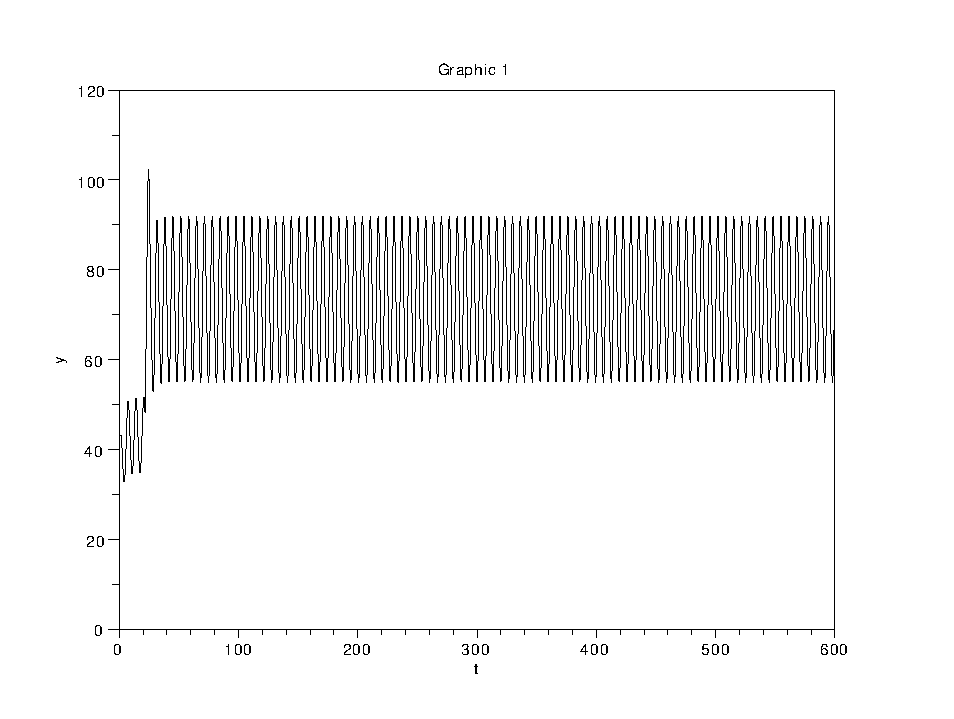
\includegraphics[scale=0.4,trim = 0cm 0cm 0cm
                            0cm, clip]
                            {./Bilder/4_1_Td_16_600s}
                              \caption{Sprungantwort PID Regler lin. Modell Totzeit $T_d = 1.6$ 600s}
                        \end{figure}
                    \end{minipage}
                
                \end{tabular}
            \end{center}
    
        Anhand der 5 Simulationen mit steigender Totzeit lässt sich erkennen, dass die Sprungantwort zunehmend
        überschwingt. Bei dieser Simulation hat der Regler keine Ahnung von der Totzeit und erwartet eine sofortige
        Reaktion auf seine Reglung. Da diese jedoch erst verspätet bei dem Regler ankommt übersteuert er. Je größer die
        Totzeit ist umso mehr fällt dieser Effekt auf. In unserem Fall schafft es der Regler für eine Totzeit von $1.6
        \ s$ nicht mehr, aus dem Überwingen rauszukommen und wir instabil.
    

    \end{quote}
    
    \subsection{Regelkreis mit PID-Regler}
    Aufgabe:\\
    Simulieren Sie den Regelkreis mit PID-Regler (ab hier immer mit Totzeit und dem vorgegebenen Scicos- Modell von der
    Webseite) unter einer sprungförmigen Referenz der Amplitude $+30^{\circ}C$ ! Kommentieren Sie kurz Ihre
    Beobachtungen!\vspace{1em}
    
    \begin{quote}
        \begin{figure}[H]
        \centering
            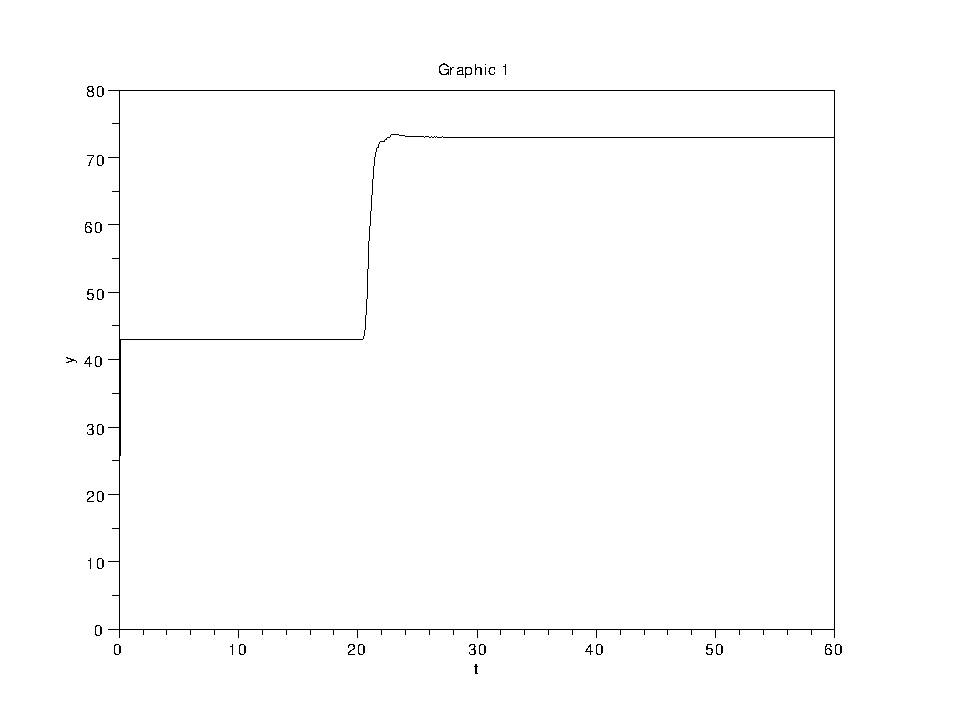
\includegraphics[scale=0.7, trim = 0cm 0cm 0cm 0cm, clip]{./Bilder/4_2_Td_04}
                \caption{Sprungantwort PID Regler nicht-lin. Modell Totzeit $T_d = 0.4$}
        \end{figure}
    
        Bei dieser Simulation wurde anstatt des linearisierten Modells der Stecke, das nichtlinearisierte Modell
        verwandt. Es fällt auf, dass dieses Modell besser die Temperatur des Arbeitspunktes ansteuern kann. Die
        Sprungantwort reagiert ein klein bisschen weniger Überschwingen als es das lineare Modelle mit der selben
        Totzeit gemacht hat.
    
    \end{quote}
    
    \subsection{Smith-Prädiktor}
    Aufgabe:\\
    Implementieren Sie ihren Smith-Prädiktor und simulieren Sie erneut! Was ändert sich, was bleibt gleich?\vspace{1em}
    
    \begin{quote}
        \begin{figure}[H]
        \centering
            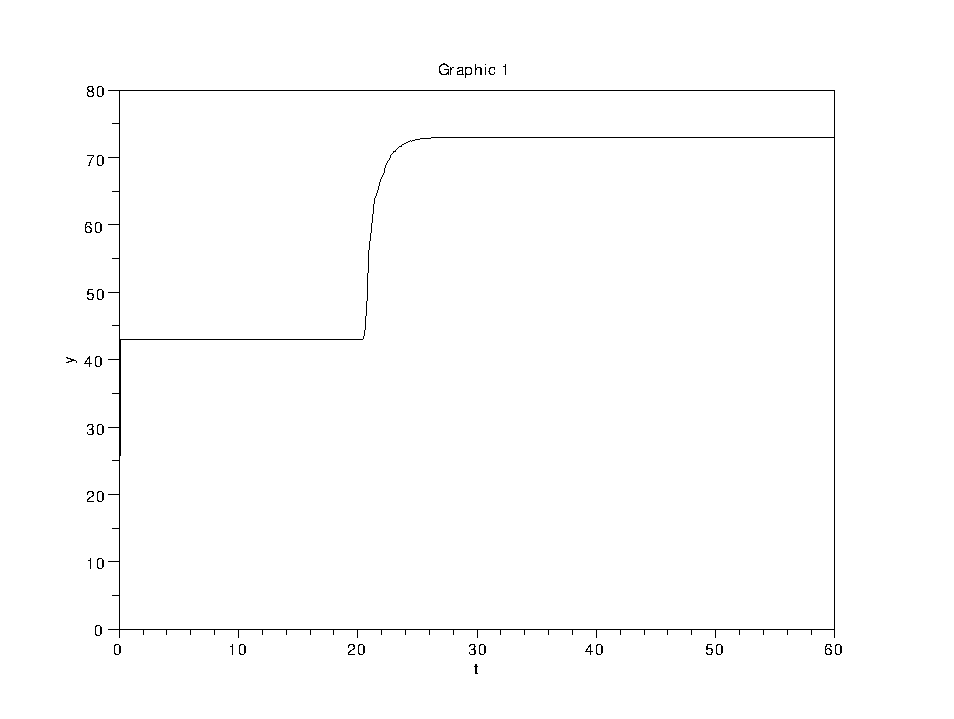
\includegraphics[scale=0.7, trim = 0cm 0cm 0cm 0cm, clip]{./Bilder/4_3_Td_04}
               \caption{Sprungantwort PID Regler nicht-lin. Modell Smith-Prädiktor Totzeit $T_d = 0.4$}
        \end{figure}
    
        Bei dieser Simulation wurde ein Smith-Prädiktor hinzugefügt. Dieser zeigt seine Aufwirkung auf die
        Sprungantwort, in dem sie weicher verläuft und auch kein bisschen mehr überschwingt. Diese Sprungantwort hat den
        bisher besten verlauf, der bis hierher betrachteten Sprungantworten.
    
    \end{quote}
    
    
    \subsection{Pad\'e-Approximation}
    Aufgabe:\\
    Implementieren Sie nun auch den Regler auf Basis der Pad\'e-Approximation und simulieren Sie einen Führungssprung
    $+30^{\circ} C$ ! Wie ist die Regelgüte im Vergleich zum PID-Regler mit Smith-Prädiktor?\vspace{1em}
    
    
    \begin{quote}
        \begin{figure}[H]
        \centering
            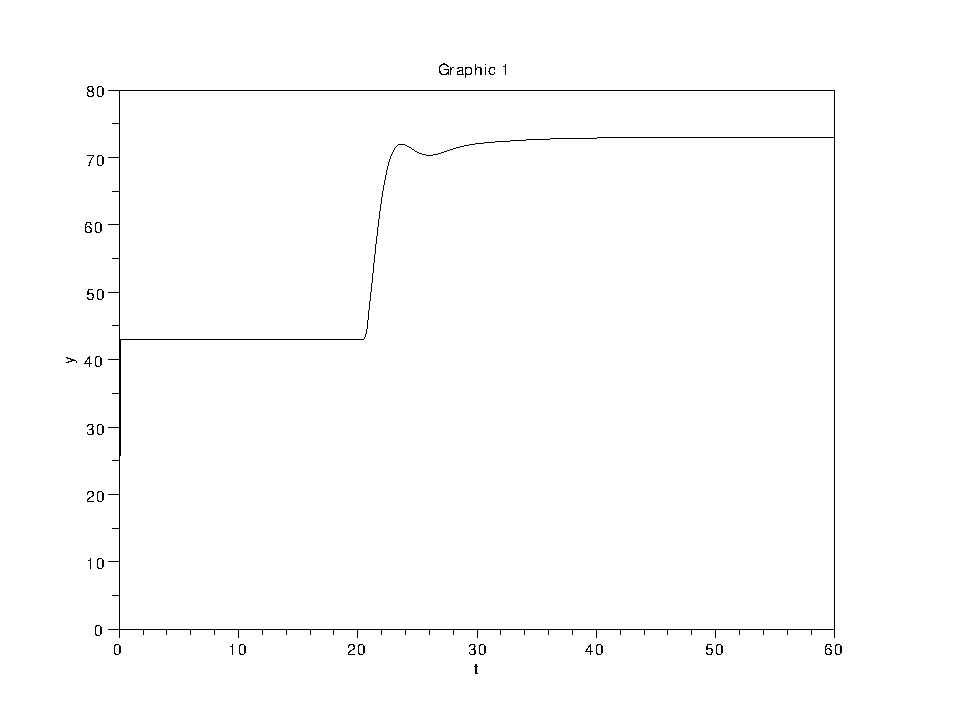
\includegraphics[scale=0.7, trim = 0cm 0cm 0cm 0cm, clip]{./Bilder/4_4_Td_04}
                \caption{Sprungantwort PID Regler Pade (KposI) nicht-lin. Modell Smith-Prädiktor Totzeit $T_d = 0.4$}
        \end{figure}
        
        Bei dem Regler mit Pad\'e Approximation verschlechtert sich das Sprungverhalten wieder auffällig. Es ist wieder
        ein überschwingen zu erkennen. Das ist auch nicht verwunderlich, da die Totzeit bei diesem Regeler nur
        angenähert wurde, während die Totzeit bei dem Smith-Prädiktor durch ein \"Delay\"-Block dargestellt wurde, der
        genauer arbeitet als die Approximation.
        
    \end{quote}
    
    
    \subsection{Führungsverhalten beim Störfall}
    Aufgabe:\\
    Erproben sie nun einen Störfall: Erhöhen Sie die Totzeit (nur die des Modells, die Regler bleiben die gleichen)
    auf $T_d = 0.7s$ und simulieren Sie erneut das Führungsverhalten beider Regelkreise! Kommentieren Sie kurz das
    Ergebnis!\vspace{1em}
    
    \begin{quote}
 
            \begin{center}
                \begin{tabular}{ll}
                
                \hspace{-1cm}
                    \begin{minipage}{0.6\textwidth}
                        \begin{figure}[H]
                            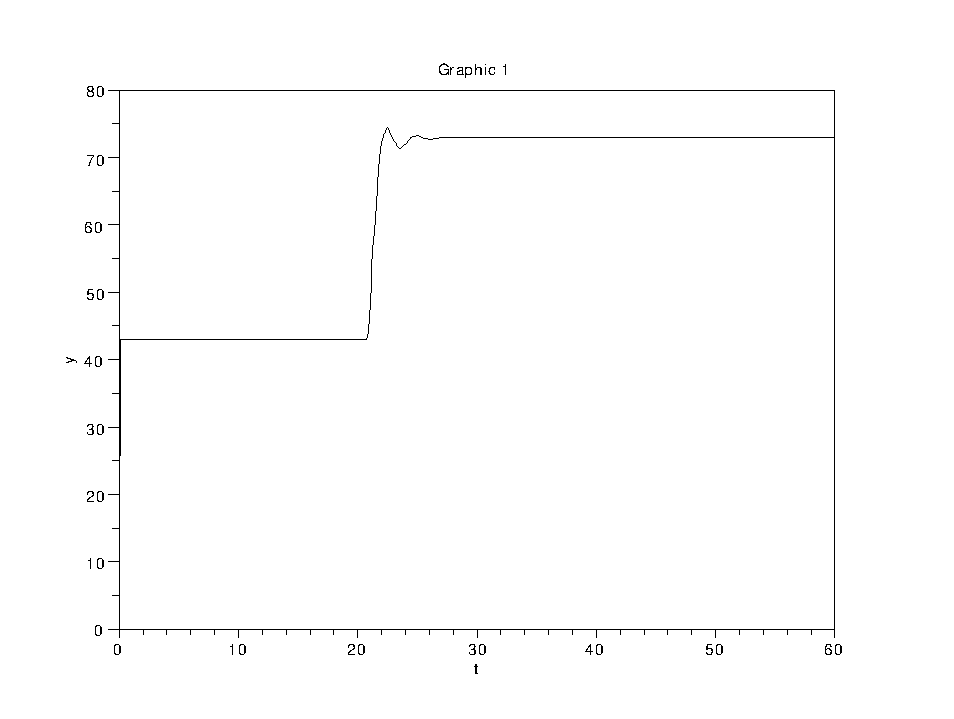
\includegraphics[scale=0.4, trim = 0cm 0cm 0cm
                            0cm, clip]
                            {./Bilder/4_5_Td_04_K_tilde}
                              \caption{Sprungantwort PID Regler lin. Modell Totzeit Strecke $T_d = 0.7$}
                        \end{figure}
                    \end{minipage}
                    
                    \begin{minipage}{0.6\textwidth}
                        \begin{figure}[H]
                            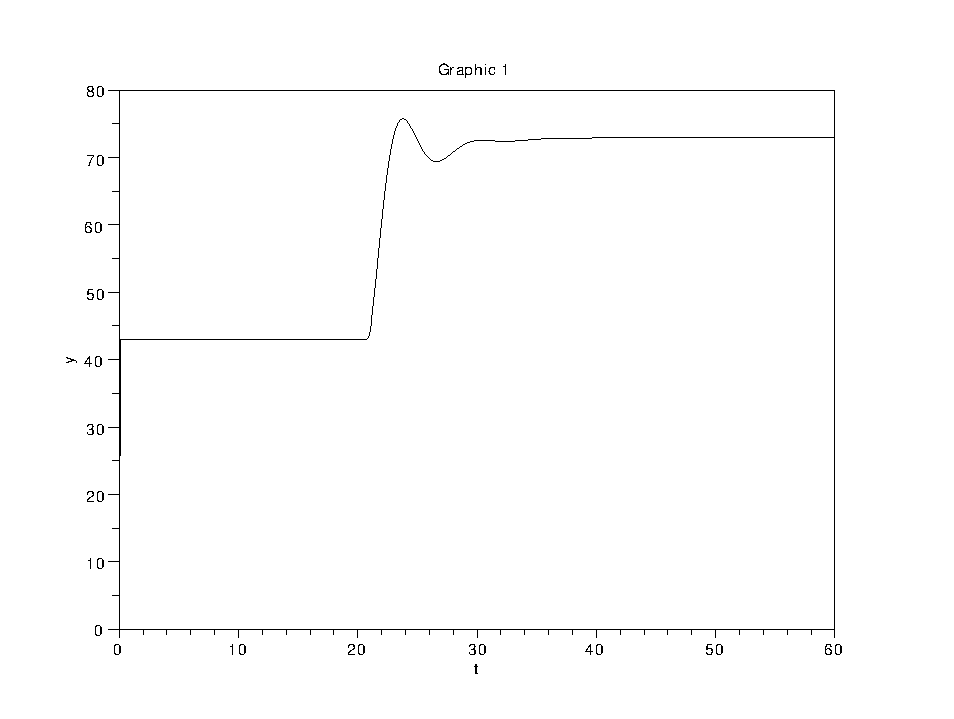
\includegraphics[scale=0.4,trim = 0cm 0cm 0cm
                            0cm, clip]
                            {./Bilder/4_5_Td_04_KposI}
                              \caption{Sprungantwort PID Regler(KposI) lin. Modell Totzeit Strecke $T_d = 0.7$ }
                        \end{figure}
                    \end{minipage}
                
                \end{tabular}
            \end{center} 
        
        
    \end{quote}
    
    
    
\end{quote}

%--------------------------------------------------------------------
%--------------------------------------------------------------------


\section{Durchführung}
\begin{quote}
    
    
    \subsection{Arbeitspunkttemperatur}
    \begin{quote}
        
    \end{quote}
    Aufgabe:\\
    Ermitteln Sie die Temperatur, die sich bei einer Heizleistung von $10$ einstellt und verwenden Sie diese als
    Arbeitspunkttemperatur!\vspace{1em}
    
    \begin{quote}
        simulation: start bei $30^{\circ}$ sprung um $31^{\circ}$
    \end{quote}
    
    \subsection{Führungssprung des PID-Reglers}
    
    Augabe:\\
    Implementieren Sie den PID-Regler (zunächst ohne Smith-Prädiktor) am Versuchsstand und führen Sie einen
    Führungssprung um $+30^{\circ} C$ aus! Die Stellgrößen als auch die Temperatur sind jeweils für jeden Versuch
    aufzuzeichen.\vspace{1em}
    
    \begin{quote}
        
    \end{quote}
    
    
    \subsection{Führungssprung mit Smith-Prädiktor}
    
    Aufgabe:\\
    Fügen Sie nun den Smith-Prädiktor hinzu und starten Sie wiederum das Experiment!\vspace{1em}
    
    \begin{quote}
        
    \end{quote}
    
    
    \subsection{Regler auf Approximationsbasis}
    
    Aufgabe:\\
    Erproben Sie ebenfalls den Regler auf Approximationsbasis!\vspace{1em}
    
    \begin{quote}
        
    \end{quote}
    
    
    \subsection{Vergleich der Messergebnisse}
    
    Aufgabe:\\
    Vergleichen Sie ihre Messergebnisse untereinander und mit den Simulationen!
    
    \begin{quote}
        
    \end{quote}
    
    
    
    
\end{quote}

%--------------------------------------------------------------------
%--------------------------------------------------------------------


\section{Auswertung}
\begin{quote}
    
\end{quote} %Ende Section Ergebnisse

%--------------------------------------------------------------------
%--------------------------------------------------------------------


\section{Scilabcode}
\begin{quote}
%     \lstinputlisting[
%         caption={Scilab-script},
%         language=scilab,
%         label=lst:scilab]
%         {./Scilab/Pendel2a.sce}


\end{quote} %Ende section

%--------------------------------------------------------------------
%--------------------------------------------------------------------    


%\begin{thebibliography}{999}
%\bibitem {Ueberschwingweite} Prof. Dr.-Ing. Raisch, Jörg; Dipl.-Ing. Hess, Anne-Katrin; Dipl.-Ing. Seel, Thomas:
%Grundlagen der Regelungstechnik - 4.Praktikum, S.5
%\bibitem {Ausregelzeit} Prof. Dr.-Ing. Raisch, Jörg; Dipl.-Ing. Hess, Anne-Katrin; Dipl.-Ing. Seel, Thomas:
%Grundlagen der Regelungstechnik - 4.Praktikum, S.5

%\usepackage{url}


%\bibitem{krachler}Christian Krachler:
%\href{http://www.krachler.com/fileadmin/user_upload/arbeiten/Reglersynthese_Christian_Krachler.pdf}{Reglersynthese nach
% dem Frequenzkennlinienverfahren}, S16, S22, 08.05.2012

%http://krachler.com/fileadmin/user\_upload/arbeiten/Reglersynthese\_Christian\_Krachler.pdf


%Name, Vorname.; evtl. Name2, Vorname2.: Titel des Dokumentes
%oder Buches, Zeitschrift/Verlag/URL (Auflage, Erscheinungsort, -jahr), ggf. Seitenzahlen
%\bibitem [Wiki10] {DigitaleMesskette2} \url{www.wikipedia.org}, Zugriff 22.03.2010
%\end{thebibliography}


\end{document}
